\documentclass{beamer}
% Use DS9 global theme
\usepackage{../../../../shared/templates/ds9_theme}

% Title page configuration
\title{Lesson CH:9}
\subtitle{Statics and Torque}
\author{Mr. Gullo}
\date{November 2024}

% Add logo
\logo{
\includegraphics[width=0.1\linewidth]{phys12-shared-cinec-logo.png}}


% Table of contents at the beginning of each section
\AtBeginSection[]
{
  \begin{frame}
    \frametitle{Table of Contents}
    \tableofcontents[currentsection]
  \end{frame}
}


\begin{document}

\frame{\titlepage}

\section{Key Concepts and Definitions}
\begin{frame}
\frametitle{Equilibrium Conditions}

\begin{block}{First Condition for Equilibrium}
\begin{itemize}
    \item Net external force must be zero ($\sum \vec{F} = \vec{0}$)
    \item Applies to both linear and rotational motion
    \item Required for absence of acceleration
\end{itemize}
\end{block}

\begin{figure}
    \centering
    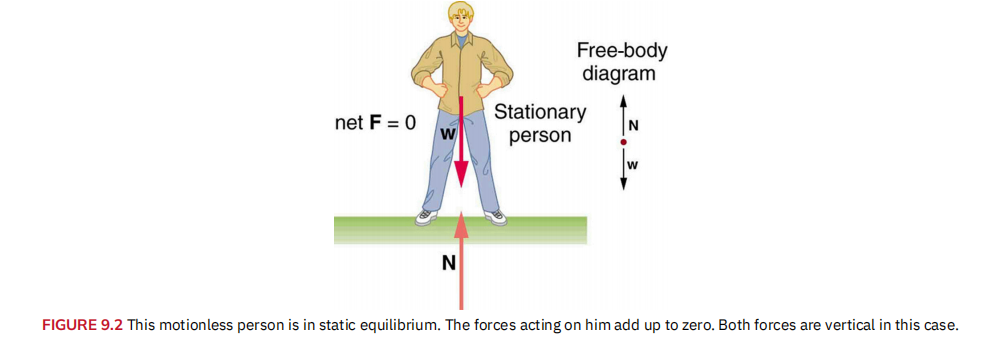
\includegraphics[width=0.8\linewidth]{Screenshot 2024-11-04 115835.png}
\end{figure}
\end{frame}

\begin{frame}
\frametitle{Torque and Rotational Equilibrium}

\begin{block}{Understanding Torque}
Torque ($\tau$) is the rotational equivalent of force:
\begin{itemize}
    \item Measures effectiveness of force in changing angular velocity
    \item Represents rotational acceleration capability
    \item Defined as: $\tau = rF\sin\theta$
    \item where:
    \begin{itemize}
        \item $r$ is distance from pivot to force application point
        \item $F$ is magnitude of force
        \item $\theta$ is angle between force and position vector
    \end{itemize}
\end{itemize}
\end{block}
\end{frame}
\begin{frame}
\begin{block}{Second Condition for Equilibrium}
\begin{itemize}
    \item Net external torque must be zero ($\sum \vec{\tau} = \vec{0}$)
    \item Torque ($\vec{\tau}$) = $rF \sin \theta$
    \item Where $\vec{r}$ is position vector from pivot point, $\vec{F}$ is force vector
    \item Perpendicular lever arm ($r_\perp$) is shortest distance from pivot to force line
\end{itemize}
\end{block}

\begin{figure}
    \centering
    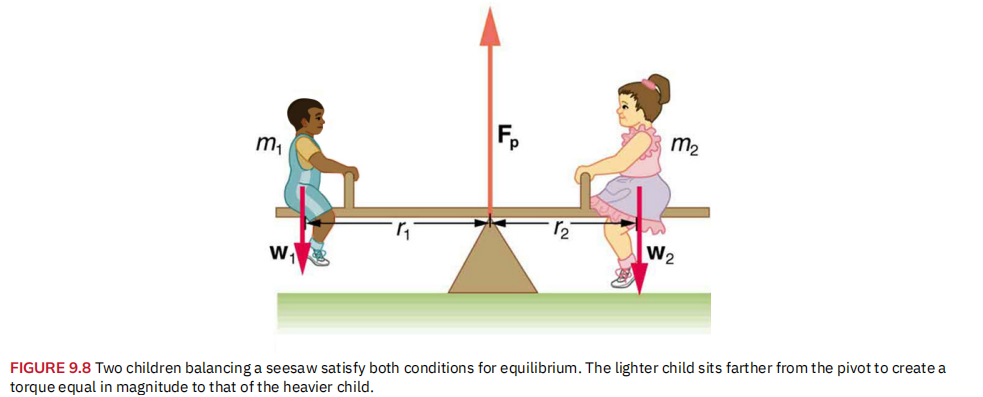
\includegraphics[width=1\linewidth]{Screenshot 2024-11-04 120123.png}
\end{figure}
\end{frame}
\begin{frame}
\frametitle{Types of Equilibrium}
\begin{itemize}
    \item \textbf{Stable Equilibrium}
    \begin{itemize}
        \item When displaced, experiences force/torque opposing displacement
        \item System returns to original position
    \end{itemize}
    \item \textbf{Unstable Equilibrium}
    \begin{itemize}
        \item When displaced, experiences force/torque in same direction as displacement
        \item System moves further from original position
    \end{itemize}
    \item \textbf{Neutral Equilibrium}
    \begin{itemize}
        \item Equilibrium independent of displacement
        \item System remains in new position when displaced
    \end{itemize}
\end{itemize}
\end{frame}

\begin{frame}
\frametitle{Simple Machines}
\begin{itemize}
    \item \textbf{Basic Principles}
    \begin{itemize}
        \item Devices that multiply or augment applied forces
        \item Trade-off between force and distance
        \item Examples: lever, nail puller, wheelbarrow, crank
    \end{itemize}
    \end{itemize}
\begin{figure}[H]
    \centering
    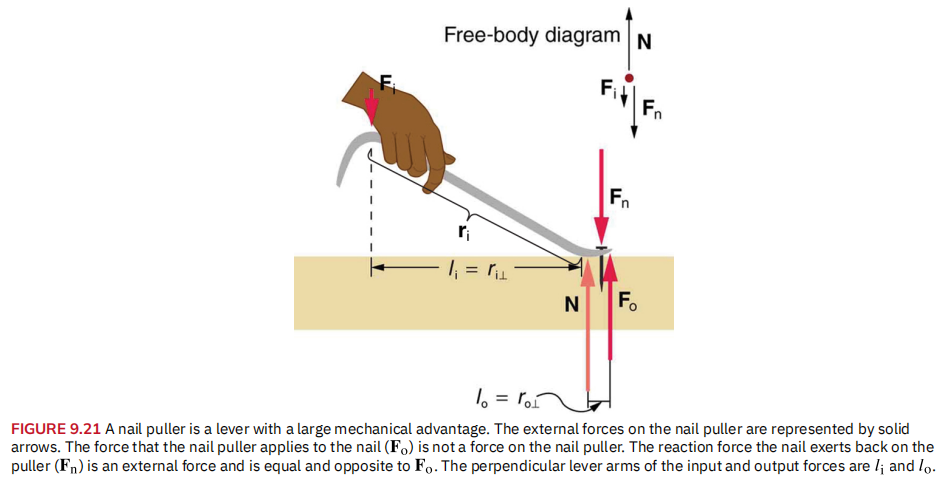
\includegraphics[width=1\linewidth]{Screenshot 2024-11-04 120252.png}
\end{figure}
    
\end{frame}



\begin{frame}
    \item \textbf{Mechanical Advantage}
    \begin{itemize}
        \item Ratio of output force to input force
        \item Key measure of machine effectiveness
    \end{itemize}
\begin{figure}[H]
    \centering
    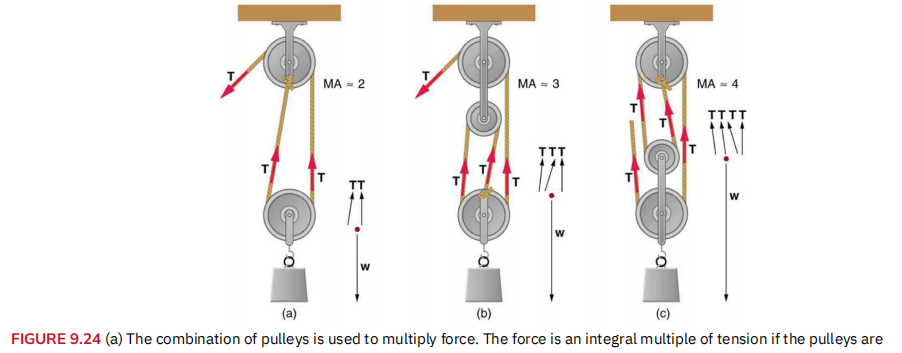
\includegraphics[width=1\linewidth]{Screenshot 2024-11-04 120504.png}
\end{figure}
    
\end{frame}

\section{Problems and Solutions}

\section{9.2 THE SECOND CONDITION FOR EQUILIBRIUM}

\begin{frame}
\frametitle{Problem 2}
When tightening a bolt, you push perpendicularly on a wrench with a force of 165 N at a distance of 0.140 m from the center of the bolt.
\begin{itemize}
    \item[(a)] How much torque are you exerting in newton $\times$ meters (relative to the center of the bolt)?
    \item[(b)] Convert this torque to foot-pounds.
\end{itemize}
\end{frame}

\begin{frame}
\frametitle{Problem 2 - Solution}
\textbf{Solution:}
\begin{itemize}
    \item[(a)] Using the torque equation $\tau = r_\perp F$:
    \begin{itemize}
        \item $\tau = 0.140 \text{ m} \times 165 \text{ N} = 23.1 \text{ N} \cdot \text{m}$
    \end{itemize}
    \item[(b)] Converting to foot-pounds:
    \begin{itemize}
        \item $\tau = 23.1 \text{ N}\cdot\text{m} \times \frac{0.738 \text{ ft}\cdot\text{lb}}{1 \text{ N}\cdot\text{m}} = 17.0 \text{ ft}\cdot\text{lb}$
    \end{itemize}
\end{itemize}
\end{frame}

\section{9.3 STABILITY}

\begin{frame}
\frametitle{Problem 10}
A 17.0-m-high and 11.0-m-long wall under construction and its bracing are shown in Figure 9.30. The wall is in stable equilibrium without the bracing but can pivot at its base. Calculate the force exerted by each of the 10 braces if a strong wind exerts a horizontal force of 650 N on each square meter of the wall. Assume that the net force from the wind acts at a height halfway up the wall and that all braces exert equal forces parallel to their lengths. Neglect the thickness of the wall.
\begin{figure}[H]
    \centering
    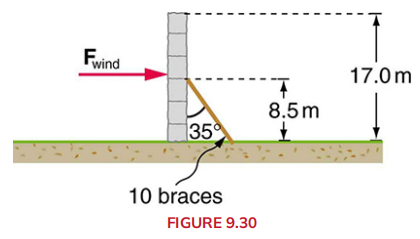
\includegraphics[width=0.7\linewidth]{Screenshot 2024-11-04 122251.png}
\end{figure}

\end{frame}

\begin{frame}
\frametitle{Problem Statement}
A wall under construction with bracing:
\begin{itemize}
    \item Wall dimensions:
    \begin{itemize}
        \item Height: 17.0 m
        \item Length: 11.0 m
    \end{itemize}
    \item Wind force: 650 N per square meter
    \item 10 braces at 35° angle
    \item Wind acts at half height
    \item Wall can pivot at base
    \item All braces exert equal forces
\end{itemize}
\textbf{Goal:} Calculate force exerted by each brace
\end{frame}

\begin{frame}
\frametitle{Problem Analysis}
\begin{itemize}
    \item Key considerations:
    \begin{itemize}
        \item Take pivot point at wall base
        \item Neglect wall thickness
        \item Forces acting:
        \begin{itemize}
            \item $$F_{brace} \times 10$$
            \item Weight of wall (w)
            \item Normal force (N)
        \end{itemize}
    \end{itemize}
    \item Using second condition for equilibrium:
    $$\text{net}\tau = 0 \Rightarrow \text{net}\tau_{\text{cw}} = -\text{net}\tau_{\text{ccw}}$$
\end{itemize}
\end{frame}

\begin{frame}
\frametitle{Mathematical Solution}
\begin{align*}
\text{net}\tau_{\text{cw}} &= -\text{net}\tau_{\text{ccw}}\\
(8.5\text{ m}) \times F_{\text{wind}} &= rF_b \times 10 = (8.5\text{ m})\sin 35^\circ \times F_b \times 10 \\
F_{\text{wind}} &= 10\sin 35^\circ F_b \\
F_b &= \frac{F_{\text{wind}}}{10\sin 35^\circ}
\end{align*}

Wind force calculation:
\begin{align*}
F_{\text{wind}} &= \frac{F}{A} \times A = 650\text{ N/m}^2 \times 11.0\text{ m} \times 17.0\text{ m} \\
&= 121,550\text{ N}
\end{align*}
\end{frame}

\begin{frame}
\frametitle{Final Result}
Therefore:
\begin{equation*}
F_b = \frac{121,550\text{ N}}{10 \times 0.5736} = 2.12 \times 10^4\text{ N}
\end{equation*}

\begin{itemize}
    \item Each brace must exert a force of 21.2 kN
    \item This significant force demonstrates:
    \begin{itemize}
        \item Importance of proper bracing in construction
        \item Impact of wind loads on tall structures
        \item Need for careful engineering calculations
    \end{itemize}
\end{itemize}
\end{frame}



\section{9.4 APPLICATIONS OF STATICS, INCLUDING PROBLEM-SOLVING STRATEGIES}


\begin{itemize}
    \item \url{https://www.youtube.com/watch?v=pK_oW62-zrc}
    \item \url{https://www.youtube.com/shorts/CxRw2n3lD7I}
    \item \url{https://www.youtube.com/shorts/sdC36VK_tY0}
\end{itemize}

\begin{frame}
\frametitle{Problem 18}
The center of gravity of a 5.0 kg pole held by a pole vaulter is 2.00 m from the left hand, and the hands are 0.700 m apart. Calculate the force exerted by:
\begin{itemize}
    \item[(a)] his right hand
    \item[(b)] his left hand
\begin{figure}[H]
    \centering
    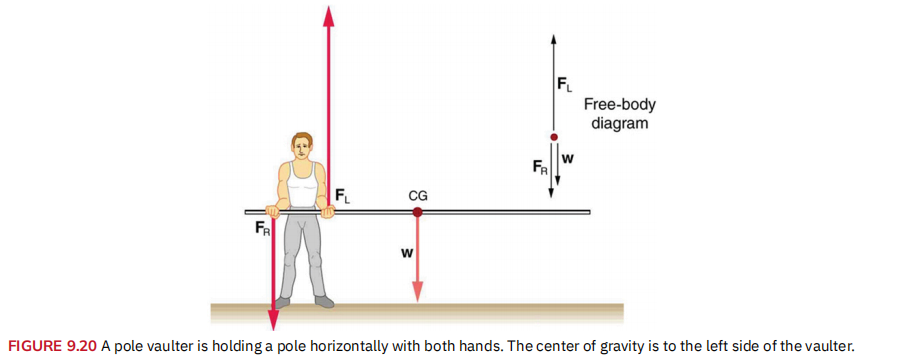
\includegraphics[width=0.5\linewidth]{Screenshot 2024-11-07 130412.png}
\end{figure}
\end{itemize}
\end{frame}

\begin{frame}
\frametitle{Problem 18 - Solution}
\textbf{Solution:}
Using the center of gravity as reference:
\begin{itemize}
    \item[(a)] Taking pivot at left hand:
    \begin{itemize}
        \item net $\tau = 0$
        \item $F_R(0.7 \text{ m}) = (5.0 \text{ kg})(9.80 \text{ m/s}^2)(2.0 \text{ m})$
        \item $F_R = 140 \text{ N}$
    \end{itemize}
    \item[(b)] Total weight must be supported:
    \begin{itemize}
        \item $F_L + F_R = (5.0 \text{ kg})(9.80 \text{ m/s}^2)$
        \item $F_L = 49 \text{ N}$
    \end{itemize}
\end{itemize}
\end{frame}

\section{9.5 SIMPLE MACHINES}

\begin{frame}
\frametitle{Problem 22}
A typical car has an axle with 2.0 cm radius driving a tire with a radius of 30.0 cm. What is its mechanical advantage assuming the very simplified model in Figure 9.23(b)?
\begin{figure}[H]
    \centering
    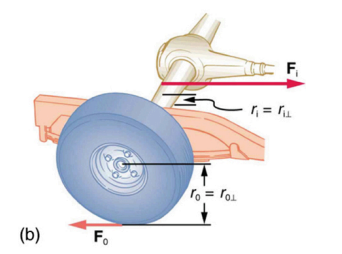
\includegraphics[width=0.7\linewidth]{Screenshot 2024-11-04 122444.png}
\end{figure}

\end{frame}

\begin{frame}
\frametitle{Problem 22 - Solution}
\textbf{Solution:}
Mechanical advantage = $r_2/r_1 = 30.0 \text{ cm}/2.0 \text{ cm} = 15$

Step-by-step explanation:
\begin{enumerate}
    \item Identify radii:
    \begin{itemize}
        \item Inner radius $(r_1) = 2.0 \text{ cm}$
        \item Outer radius $(r_2) = 30.0 \text{ cm}$
    \end{itemize}
    \item Calculate mechanical advantage:
    \begin{itemize}
      \item \mathrm{MA}=\frac{F_{\mathrm{o}}}{F_{\mathrm{i}}}=\frac{l_{\mathrm{i}}}{l_{\mathrm{o}}} .
        \item $\text{MA} = r_2/r_1$
        \item $\text{MA} = 30.0/2.0 = 15$
    \end{itemize}
\end{enumerate}
\end{frame}

\section{9.6 FORCES AND TORQUES IN MUSCLES AND JOINTS}

\begin{frame}
\frametitle{Problem 26}
Verify that the force in the elbow joint in Example 9.4 is 407 N, as stated in the text.
\begin{figure}
    \centering
    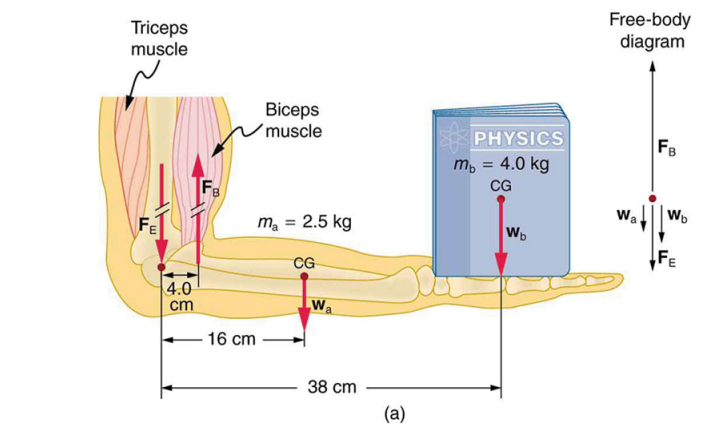
\includegraphics[width=0.7\linewidth]{Screenshot 2024-11-04 122655.png}
    \caption{FIGURE 9.25 (a) The figure shows the forearm of a person holding a book. The biceps exert a force $\mathbf{F}_{\mathrm{B}}$ to support the weight of the forearm and the book. The triceps are assumed to be relaxed.}
\end{figure}
\end{frame}

\begin{frame}
\begin{figure}
    \centering
    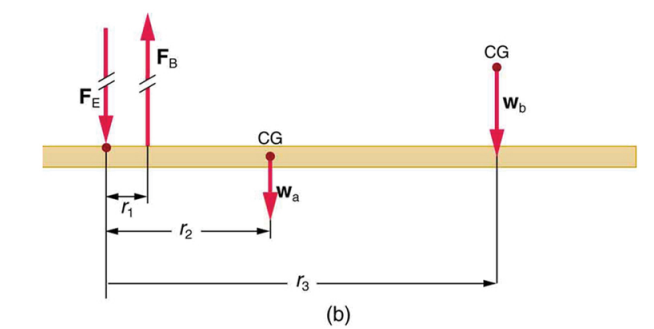
\includegraphics[width=0.7\linewidth]{Screenshot 2024-11-04 122703.png}
    \caption{ (b) Here, you can view an approximately equivalent mechanical system with the pivot at the elbow joint as seen in Example 9.4.}
\end{figure}
\end{frame}

\begin{frame}
\frametitle{Problem Statement}
\textbf{Problem 26:} Verify that the force in the elbow joint in Example 9.4 is 407 N.

\begin{block}{Given Values}
\begin{align*}
F_{\text{B}} &= 470 \text{ N} & r_1 &= 4.00 \text{ cm} \\
m_{\text{a}} &= 2.50 \text{ kg} & r_2 &= 16.0 \text{ cm} \\
m_{\text{b}} &= 4.00 \text{ kg} & r_3 &= 38.0 \text{ cm}
\end{align*}
\end{block}
\end{frame}


\begin{frame}
\frametitle{Detailed Derivation}

Starting from torque balance(second condition of equilibrium):
\begin{align*}
\tau_{\text{Bicep}}=\tau_{\text{arm}}+\tau_{\text{book}} \\
F_B r_1 &= w_a r_2 + w_B r_3
\end{align*}

Solving for $F_B$:
\begin{align*}
F_B &= \frac{w_a r_2 + w_B r_3}{r_1}
\end{align*}

For equilibrium of forces(first condition of equilibrium):
\begin{align*}
F_e &= w_a + w_B - F_B \\
&= w_a + w_B - \frac{w_a r_2 + w_B r_3}{r_1} \\
&= w_a\left(1 - \frac{r_2}{r_1}\right) + w_B\left(1 - \frac{r_3}{r_1}\right) \\
&= w_a\left(\frac{r_2}{r_1} - 1\right) + w_B\left(\frac{r_3}{r_1} - 1\right)
\end{align*}
\end{frame}
\begin{frame}
Multiply both sides by $r_1$:
\begin{equation*}
F_e \times r_1 = w_a\left(\frac{r_2}{r_1} - 1\right) + w_B\left(\frac{r_3}{r_1} - 1\right)
\end{equation*}
\end{frame}

\begin{frame}
\frametitle{Calculation}
Substituting the values:
\begin{align*}
F_E \times r_1 &= (2.50 \text{ kg})(9.80 \text{ m/s}^2)\left(\frac{16.0 \text{ cm}}{4.0 \text{ cm}}-1\right) \\
&+ (4.00 \text{ kg})(9.80 \text{ m/s}^2)\left(\frac{38.0 \text{ cm}}{4.00 \text{ cm}}-1\right)
\end{align*}

\begin{block}{Final Result}
Therefore:
\[F_E = 407 \text{ N}\]
This verifies the stated value in Example 9.4
\end{block}
\end{frame}

\end{document}